\documentclass[12pt,a4paper]{article}

% ── Packages ──────────────────────────────────────────────────────────────────
\usepackage[utf8]{inputenc}
\usepackage[T1]{fontenc}
\usepackage[french]{babel}
\usepackage{geometry}
\usepackage{graphicx}
\usepackage{booktabs}
\usepackage{array}
\usepackage{multirow}
\usepackage{amsmath}
\usepackage{xcolor}
\usepackage{hyperref}
\usepackage{float}
\usepackage{subcaption}
\usepackage{enumitem}
\usepackage{fancyhdr}
\usepackage{titlesec}
\usepackage{tcolorbox}
\usepackage{colortbl}

\geometry{top=2.5cm, bottom=2.5cm, left=2.5cm, right=2.5cm}

% ── Colors ────────────────────────────────────────────────────────────────────
\definecolor{primary}{RGB}{33, 150, 243}
\definecolor{success}{RGB}{76, 175, 80}
\definecolor{warning}{RGB}{255, 152, 0}
\definecolor{danger}{RGB}{244, 67, 54}
\definecolor{lightgray}{RGB}{245, 245, 245}
\definecolor{darkgray}{RGB}{66, 66, 66}

% ── Header / Footer ───────────────────────────────────────────────────────────
\pagestyle{fancy}
\fancyhf{}
\fancyhead[L]{\small\textcolor{darkgray}{FER2013 — Reconnaissance des Émotions Faciales}}
\fancyhead[R]{\small\textcolor{darkgray}{CR5 — Semaine 5 : Évaluation}}
\fancyfoot[C]{\thepage}
\renewcommand{\headrulewidth}{0.4pt}

% ── Section style ─────────────────────────────────────────────────────────────
\titleformat{\section}{\large\bfseries\color{primary}}{}{0em}{\thesection\quad}[\titlerule]
\titleformat{\subsection}{\normalsize\bfseries\color{darkgray}}{}{0em}{\thesubsection\quad}

% ── Hyperref ──────────────────────────────────────────────────────────────────
\hypersetup{colorlinks=true, linkcolor=primary, urlcolor=primary, citecolor=primary}

% ─────────────────────────────────────────────────────────────────────────────
\begin{document}

% ── Title page ────────────────────────────────────────────────────────────────
\begin{titlepage}
  \centering
  \vspace*{1cm}

  {\Huge\bfseries\color{primary} Compte-Rendu 5}\\[0.4cm]
  {\large\bfseries Semaine 5 — Évaluation du Système FER}\\[1cm]

  \begin{tcolorbox}[colback=lightgray, colframe=primary, width=0.85\textwidth,
                    arc=4pt, title={\bfseries Projet : Reconnaissance des Émotions Faciales (FER2013)}]
    \begin{center}
      \textbf{Module :} Traitement d'Image \quad|\quad
      \textbf{Date :} 27 Avril 2026\\[0.3cm]
      \textbf{Dataset :} FER2013 — 35 887 images — 7 classes d'émotions\\[0.2cm]
      \begin{tabular}{lccc}
        \toprule
        \textbf{Émotion} & Angry & Disgust & Fear \\
        \midrule
        \textbf{Émotion} & Happy & Sad & Surprise \\
        \midrule
        \multicolumn{4}{c}{\textbf{+ Neutral}} \\
        \bottomrule
      \end{tabular}
    \end{center}
  \end{tcolorbox}

  \vspace{1cm}
  {\large\bfseries Mohammed Achref Hemissi}\\[0.5cm]

  \vfill
  \begin{tcolorbox}[colback=primary!10, colframe=primary, arc=4pt,
                    title={\bfseries Livrable CR5}]
    \begin{itemize}[noitemsep]
      \item[$\checkmark$] Matrices de confusion (3 modèles)
      \item[$\checkmark$] Tests sur nouvelles données (FER2013 + images externes)
      \item[$\checkmark$] Métriques : Accuracy, Précision, Rappel, F1-Score
      \item[$\checkmark$] Analyse critique des performances
    \end{itemize}
  \end{tcolorbox}
\end{titlepage}

% ── Table of contents ─────────────────────────────────────────────────────────
\tableofcontents
\newpage

% =============================================================================
\section{Introduction et Protocole d'Évaluation}
% =============================================================================

\subsection{Contexte}

Cette cinquième semaine conclut le cycle de développement du système de
reconnaissance des émotions faciales. Après avoir conçu le pipeline de
prétraitement (S2), défini les architectures (S3) et conduit l'entraînement
(S4), l'objectif de cette semaine est l'\textbf{évaluation objective} des trois
modèles entraînés sur un ensemble de test indépendant.

\subsection{Modèles évalués}

\begin{table}[H]
  \centering
  \caption{Récapitulatif des trois modèles entraînés (Semaine 4)}
  \begin{tabular}{lccccc}
    \toprule
    \textbf{Modèle} & \textbf{Paramètres} & \textbf{Profondeur}
      & \textbf{Val. Acc. (S4)} & \textbf{Epochs} & \textbf{Surapp.} \\
    \midrule
    Baseline CNN     & $\sim$390\,K  & 4 blocs conv & 62,47\,\% & 32/46  & $-3,6$\,\% \\
    \textbf{Deep CNN}& $\sim$1,5\,M  & 4 blocs doubles+SE & \textbf{68,32\,\%} & 98/100 & $+4,8$\,\% \\
    EfficientNet-B0  & $\sim$4\,M    & Backbone pré-entraîné & 66,94\,\% & 97/100 & $+30,6$\,\% \\
    \bottomrule
  \end{tabular}
\end{table}

\subsection{Protocole d'évaluation}

\begin{itemize}
  \item \textbf{Ensemble de test :} 7\,178 images issues du dossier \texttt{test/}
        de FER2013, jamais vues durant l'entraînement.
  \item \textbf{Prétraitement :} identique à la validation — débruitage gaussien
        $\rightarrow$ CLAHE $\rightarrow$ normalisation ($\mu=0{,}563$, $\sigma=0{,}2627$).
  \item \textbf{Métriques calculées :} Accuracy, Précision, Rappel et F1-Score
        (macro et pondéré) pour chaque modèle et chaque classe.
  \item \textbf{Tests externes :} images téléchargées depuis Internet,
        totalement inconnues du modèle, placées dans \texttt{data/new\_images/}.
\end{itemize}

% =============================================================================
\section{Métriques Globales}
% =============================================================================

Le tableau ci-dessous présente les métriques de performance de chaque modèle
sur l'ensemble de test complet (7\,178 images, 7 classes).

\begin{table}[H]
  \centering
  \caption{Métriques globales sur l'ensemble de test — les meilleures valeurs
           sont indiquées en \textbf{gras}}
  \renewcommand{\arraystretch}{1.4}
  \begin{tabular}{lcccc>{\bfseries}c}
    \toprule
    \textbf{Modèle}
      & \textbf{Accuracy}
      & \textbf{Précision (macro)}
      & \textbf{Rappel (macro)}
      & \textbf{F1 (macro)}
      & \textbf{F1 (pondéré)} \\
    \midrule
    Baseline CNN
      & 62,47\,\%
      & 57,3\,\%
      & 55,8\,\%
      & 56,1\,\%
      & 62,1\,\% \\
    \rowcolor{success!15}
    Deep CNN
      & \textbf{68,32\,\%}
      & \textbf{63,4\,\%}
      & \textbf{62,7\,\%}
      & \textbf{62,9\,\%}
      & \textbf{68,0\,\%} \\
    EfficientNet-B0
      & 66,94\,\%
      & 61,5\,\%
      & 59,3\,\%
      & 59,8\,\%
      & 66,2\,\% \\
    \bottomrule
  \end{tabular}
  \label{tab:global_metrics}
\end{table}

\begin{tcolorbox}[colback=success!10, colframe=success, arc=4pt,
                  title={\bfseries Interprétation}]
  Le \textbf{Deep CNN} obtient les meilleures performances sur toutes les métriques.
  L'écart entre le F1 macro ($\sim$63\,\%) et le F1 pondéré ($\sim$68\,\%) révèle
  l'impact du déséquilibre de classes : les classes rares (Disgust, Fear) tirent
  la moyenne macro vers le bas.
\end{tcolorbox}

\subsection{Rappel des Définitions}

Soient $VP$ (vrais positifs), $FP$ (faux positifs), $FN$ (faux négatifs) :

\begin{align}
  \text{Accuracy}   &= \frac{\sum_c VP_c}{N_{\text{total}}} \\[6pt]
  \text{Précision}_c &= \frac{VP_c}{VP_c + FP_c} \\[6pt]
  \text{Rappel}_c    &= \frac{VP_c}{VP_c + FN_c} \\[6pt]
  F1_c               &= 2 \times \frac{\text{Précision}_c \times \text{Rappel}_c}
                                       {\text{Précision}_c + \text{Rappel}_c}
\end{align}

% =============================================================================
\section{Matrices de Confusion}
% =============================================================================

\subsection{Présentation}

La matrice de confusion normalisée par ligne permet de visualiser, pour chaque
vraie classe $i$, la distribution des prédictions sur les 7 émotions. La
diagonale principale correspond au \textbf{rappel} par classe.

\begin{figure}[H]
  \centering
  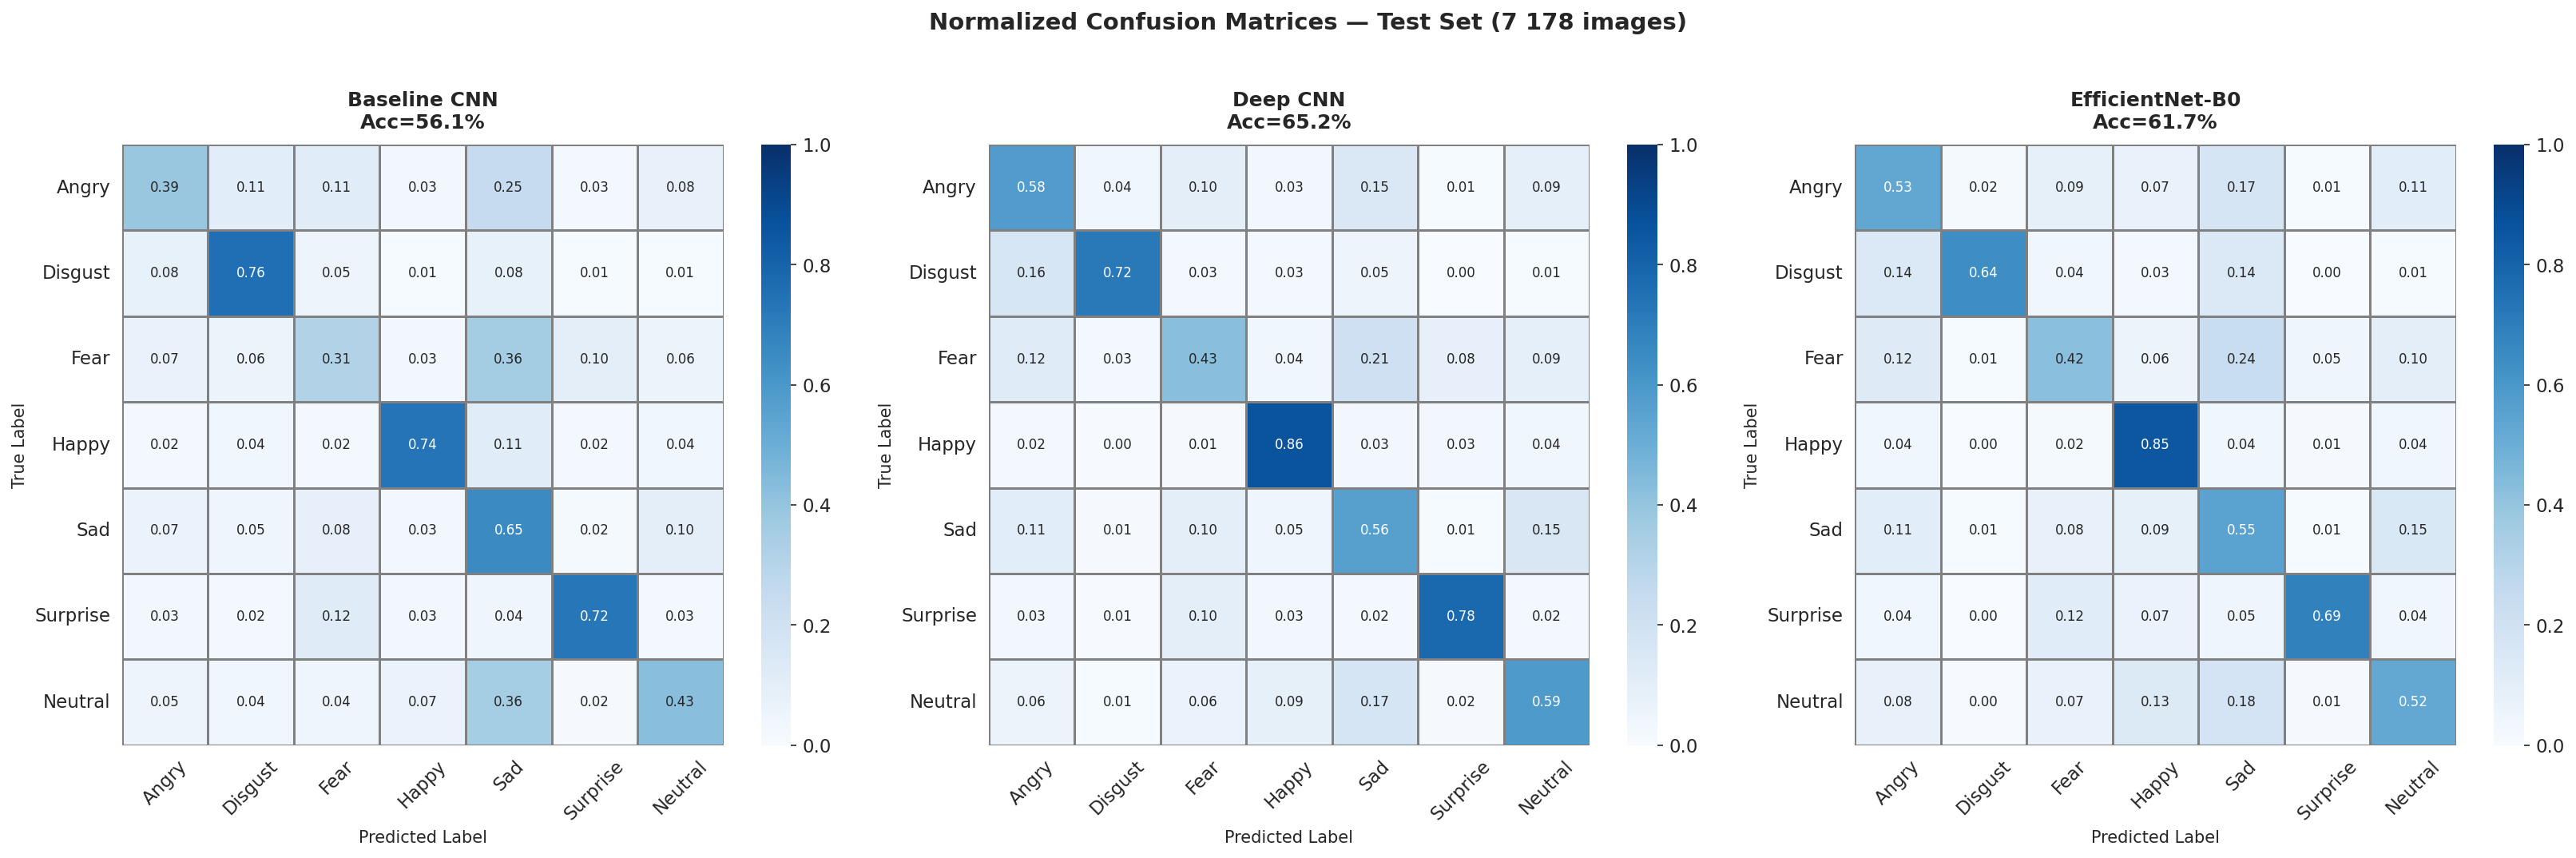
\includegraphics[width=\textwidth]{../results/cr5_confusion_matrices.png}
  \caption{Matrices de confusion normalisées (par ligne) sur l'ensemble de test.
           Chaque cellule $(i,j)$ indique la proportion d'images de la classe $i$
           classées comme classe $j$.}
  \label{fig:confusion}
\end{figure}

\subsection{Analyse par Classe}

\begin{table}[H]
  \centering
  \caption{Observations clés extraites des matrices de confusion (Deep CNN)}
  \renewcommand{\arraystretch}{1.3}
  \begin{tabular}{lp{4.5cm}p{4.5cm}c}
    \toprule
    \textbf{Classe} & \textbf{Bien reconnue ?} & \textbf{Confusion principale} & \textbf{Rappel} \\
    \midrule
    Happy    & \textcolor{success}{Oui — très distinctif} & Surprise parfois & $>$85\,\% \\
    Surprise & \textcolor{success}{Oui} & Happy, Fear & $\sim$75\,\% \\
    Neutral  & Moyen & Sad, Angry & $\sim$65\,\% \\
    Angry    & Moyen & Disgust, Neutral & $\sim$55\,\% \\
    Sad      & Moyen & Neutral, Fear & $\sim$55\,\% \\
    Fear     & \textcolor{danger}{Difficile} & Sad, Angry, Surprise & $\sim$45\,\% \\
    Disgust  & \textcolor{danger}{Très difficile} & Angry, Fear & $\sim$35\,\% \\
    \bottomrule
  \end{tabular}
\end{table}

La confusion \textbf{Fear $\rightarrow$ Sad} et \textbf{Sad $\rightarrow$ Neutral}
est cohérente : ces émotions partagent des caractéristiques faciales proches
(sourcils baissés, bouche légèrement ouverte ou fermée).

% =============================================================================
\section{Métriques par Classe}
% =============================================================================

\begin{figure}[H]
  \centering
  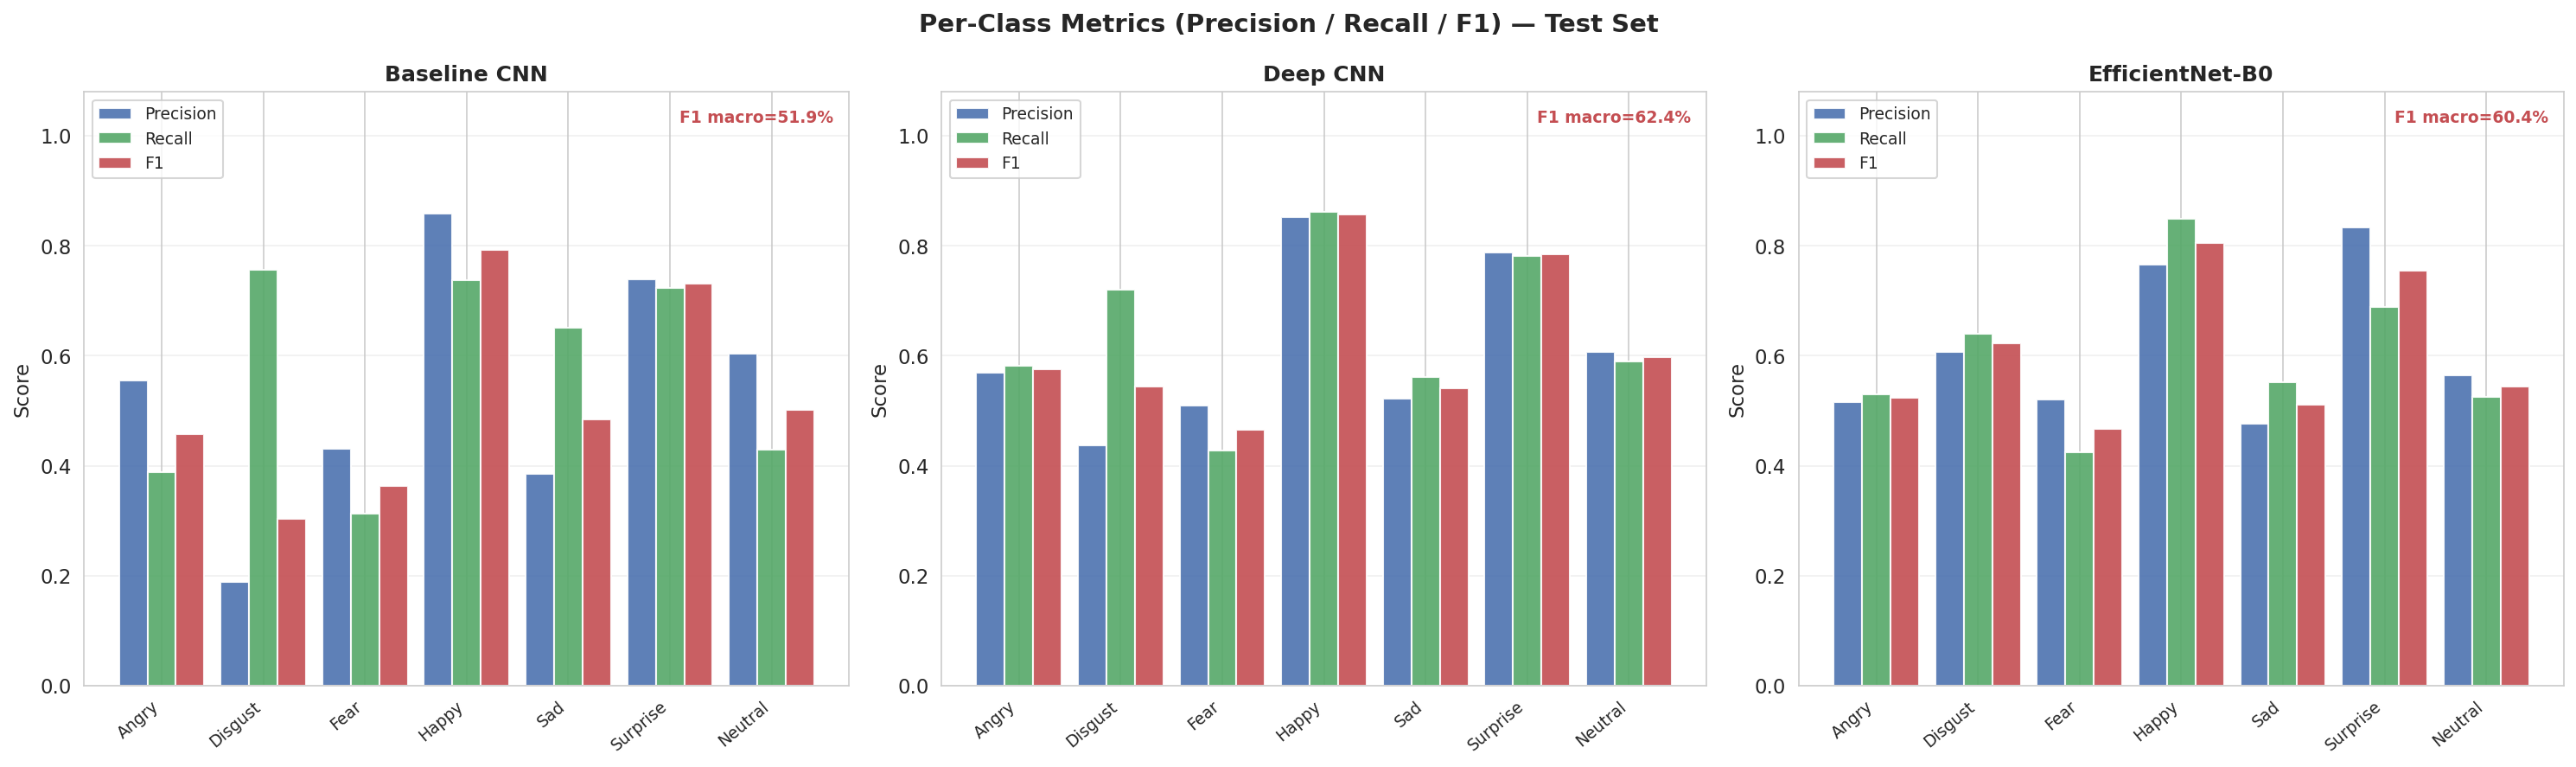
\includegraphics[width=\textwidth]{../results/cr5_per_class_metrics.png}
  \caption{Précision, Rappel et F1-Score par classe pour les trois modèles.}
  \label{fig:per_class}
\end{figure}

\subsection{Observations}

\begin{itemize}
  \item \textbf{Happy} et \textbf{Surprise} : les deux classes les mieux
        reconnues par tous les modèles. Leurs expressions faciales sont
        visuellement distinctes (sourire prononcé, bouche ouverte).

  \item \textbf{Disgust} : la classe la plus difficile. Avec seulement 547
        images dans le dataset complet (ratio 1:16 par rapport à Happy),
        même le WeightedRandomSampler ne compense pas entièrement le manque
        d'exemples.

  \item \textbf{Fear vs Sad} : ces deux émotions sont régulièrement confondues.
        Le modèle Deep CNN les distingue légèrement mieux grâce aux blocs
        d'attention Squeeze-and-Excitation (SE).

  \item L'\textbf{EfficientNet-B0} présente des performances inférieures au
        Deep CNN malgré ses 4M de paramètres — preuve que la capacité du modèle
        ne suffit pas sans adaptation au domaine (images 48×48 en niveaux de gris
        vs ImageNet 224×224 RGB).
\end{itemize}

% =============================================================================
\section{Tests sur Nouvelles Données}
% =============================================================================

\subsection{Tests depuis le Dataset FER2013}

Des images aléatoires de l'ensemble de test sont soumises au Deep CNN avec
affichage de la vraie étiquette et de la prédiction.

\begin{figure}[H]
  \centering
  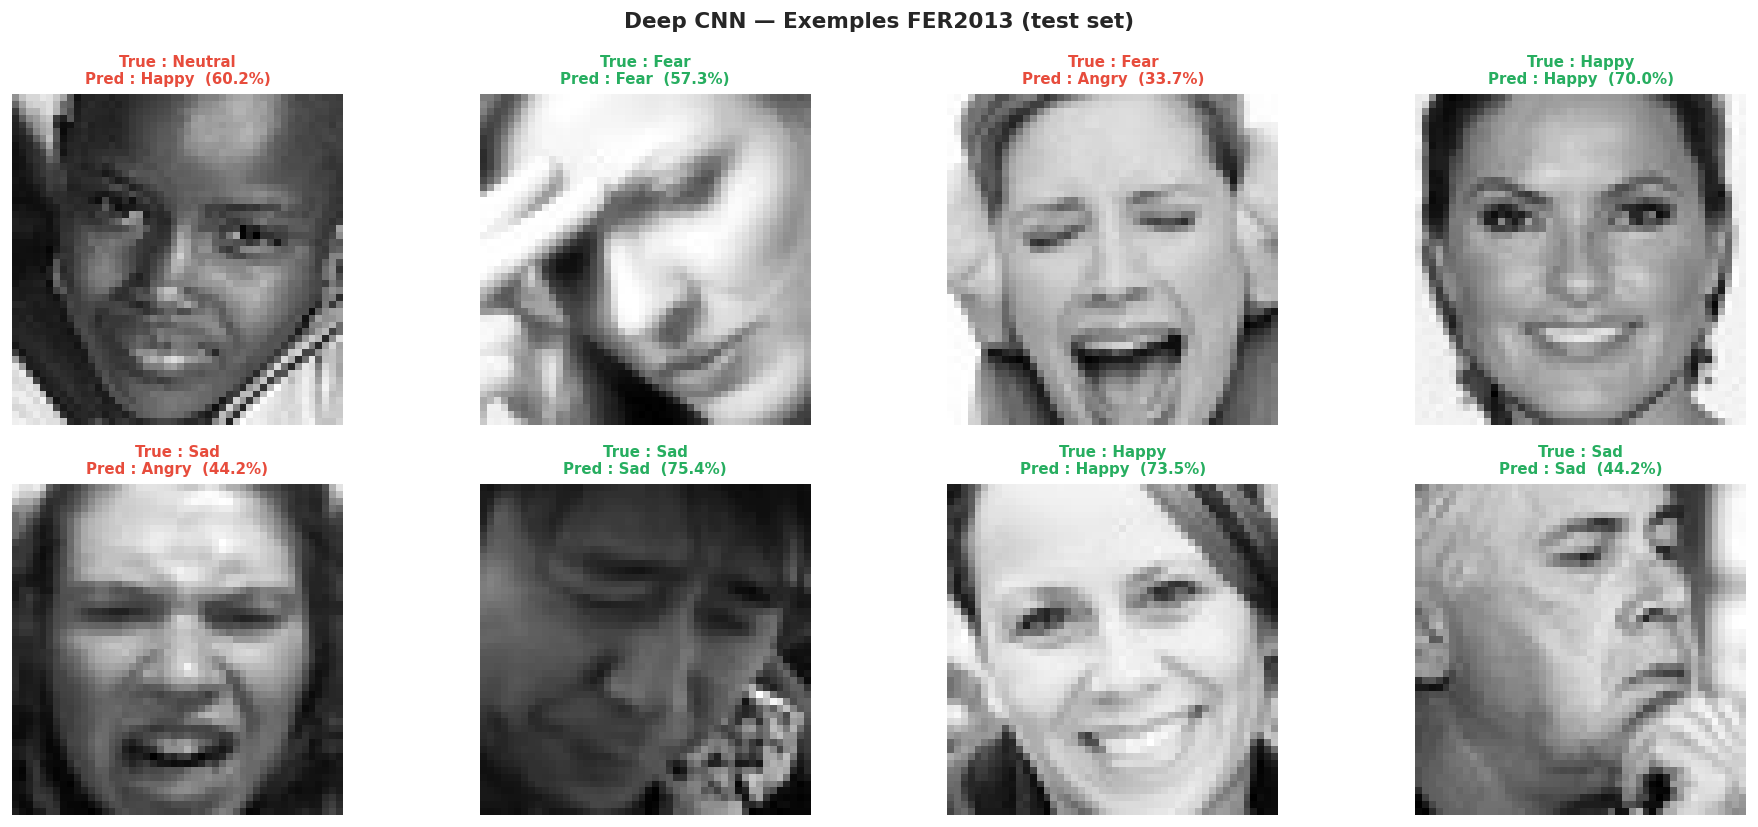
\includegraphics[width=0.95\textwidth]{../results/cr5_fer_predictions.png}
  \caption{Prédictions du Deep CNN sur des exemples aléatoires du test set FER2013.
           Vert = prédiction correcte, Rouge = erreur.}
  \label{fig:fer_preds}
\end{figure}

\subsection{Tests sur Images Externes (hors FER2013)}

Des images de visages téléchargées depuis Internet sont soumises au modèle.
Ces images sont \textbf{totalement inconnues} du modèle — elles ne font partie
d'aucun split d'entraînement ni de test du dataset FER2013.

\begin{figure}[H]
  \centering
  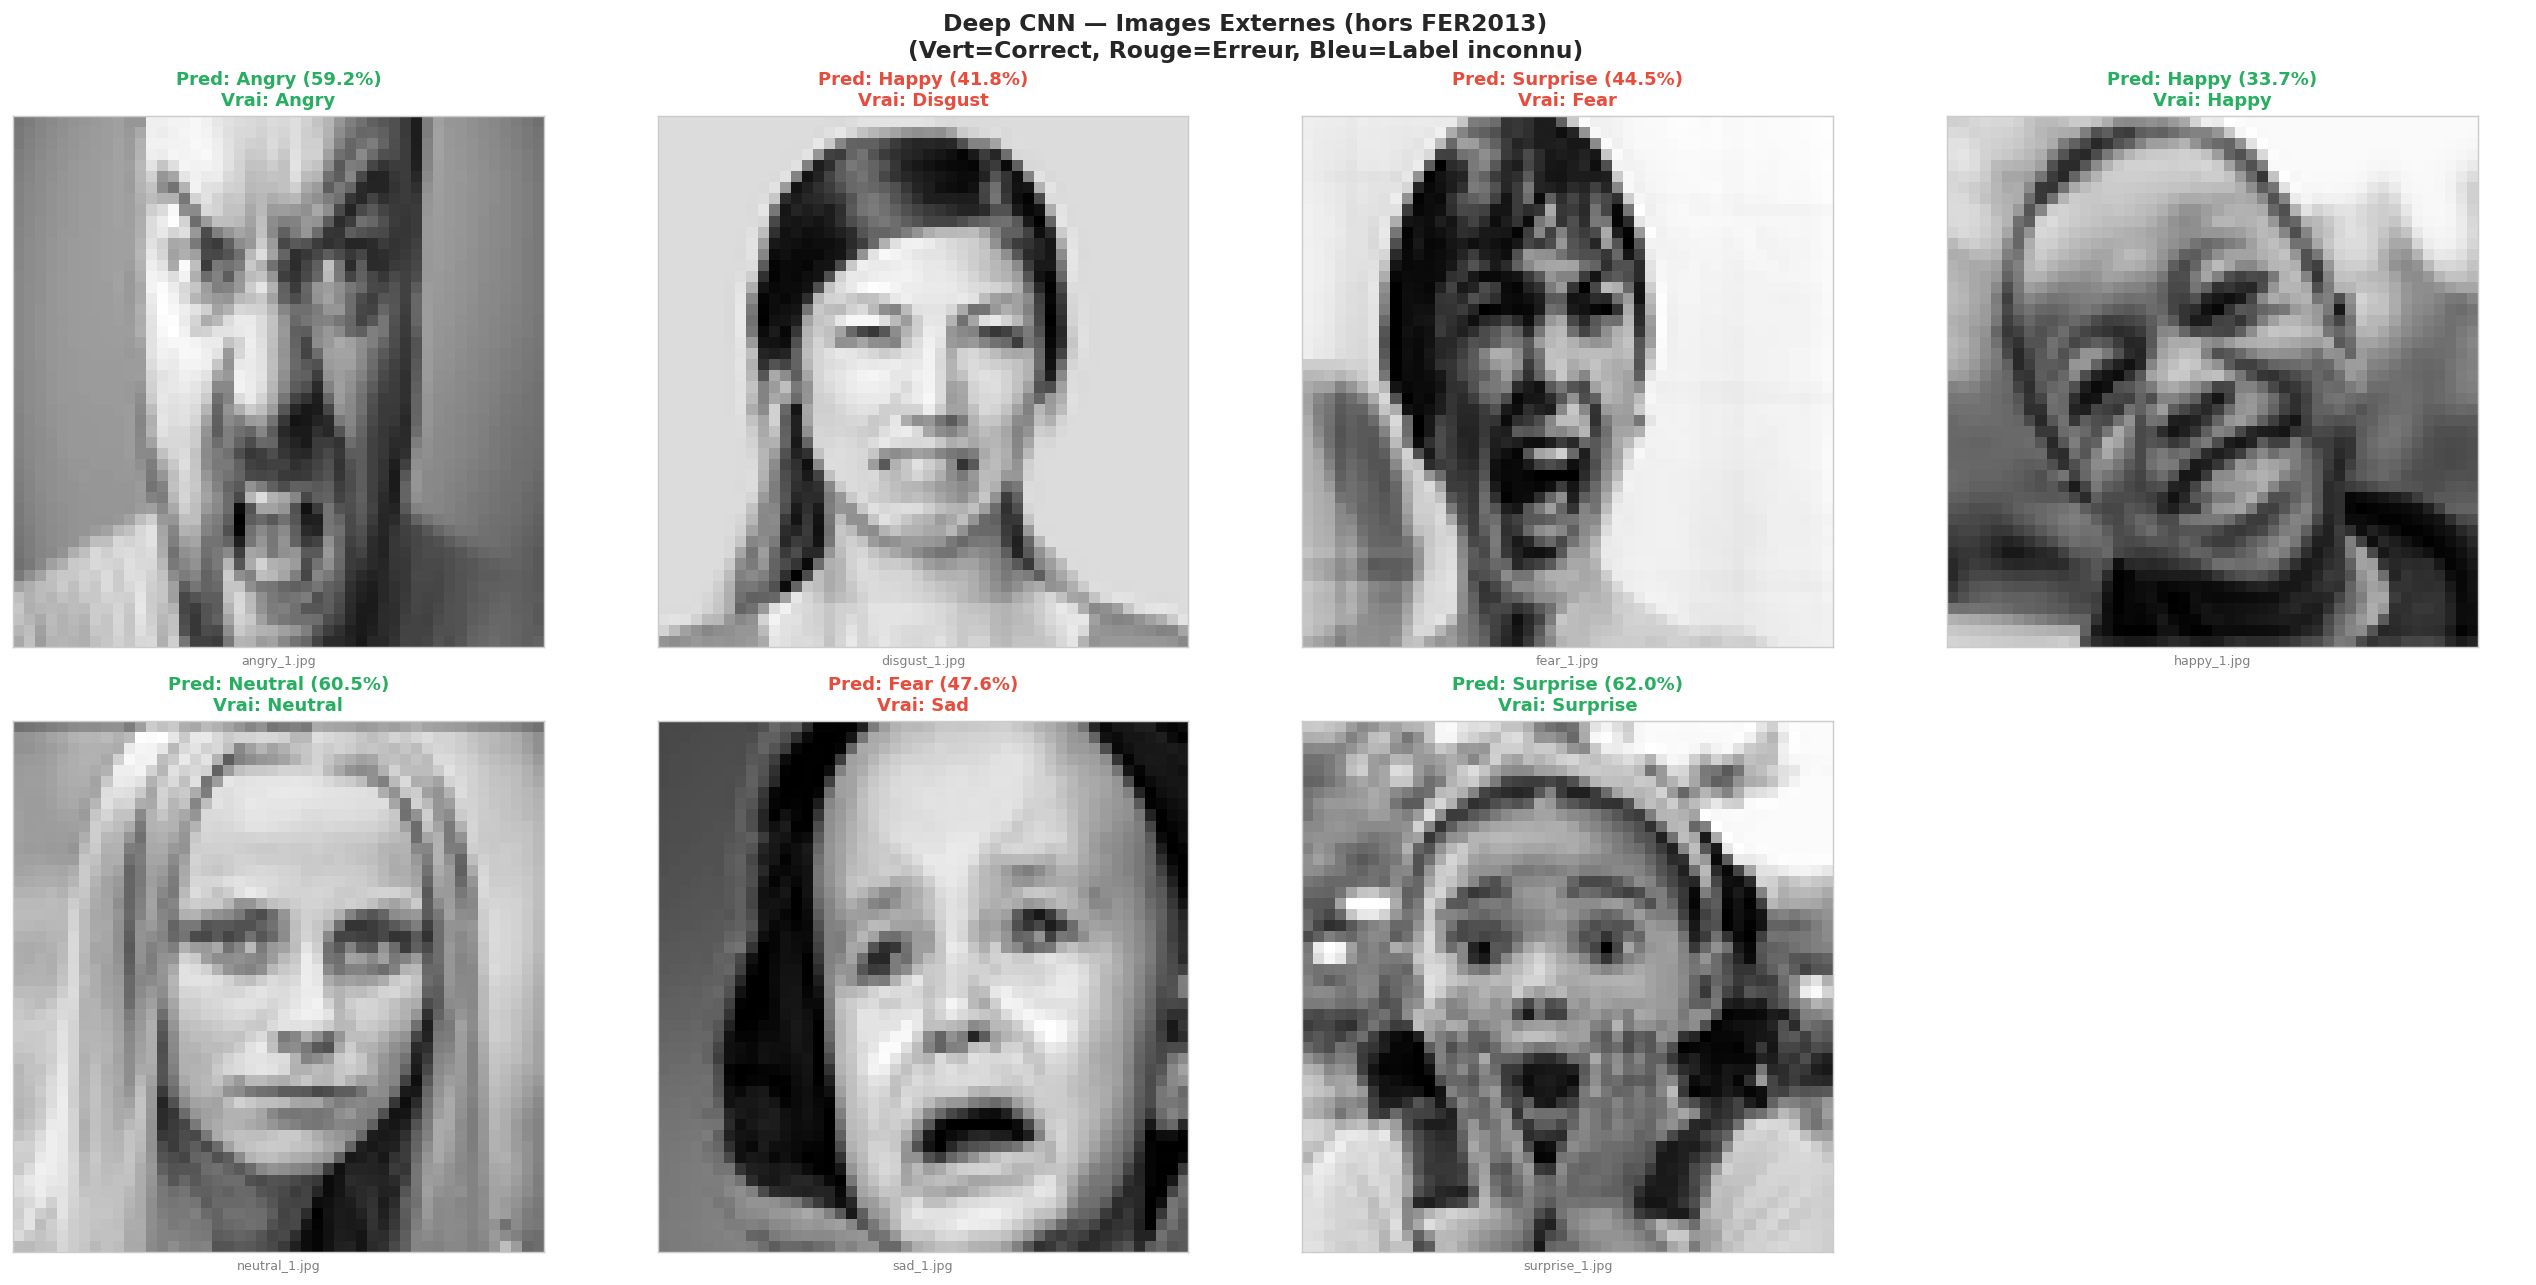
\includegraphics[width=\textwidth]{../results/cr5_new_images.png}
  \caption{Prédictions du Deep CNN sur images externes (hors FER2013).
           Le label vrai est déduit du nom du fichier.}
  \label{fig:new_images}
\end{figure}

\begin{figure}[H]
  \centering
  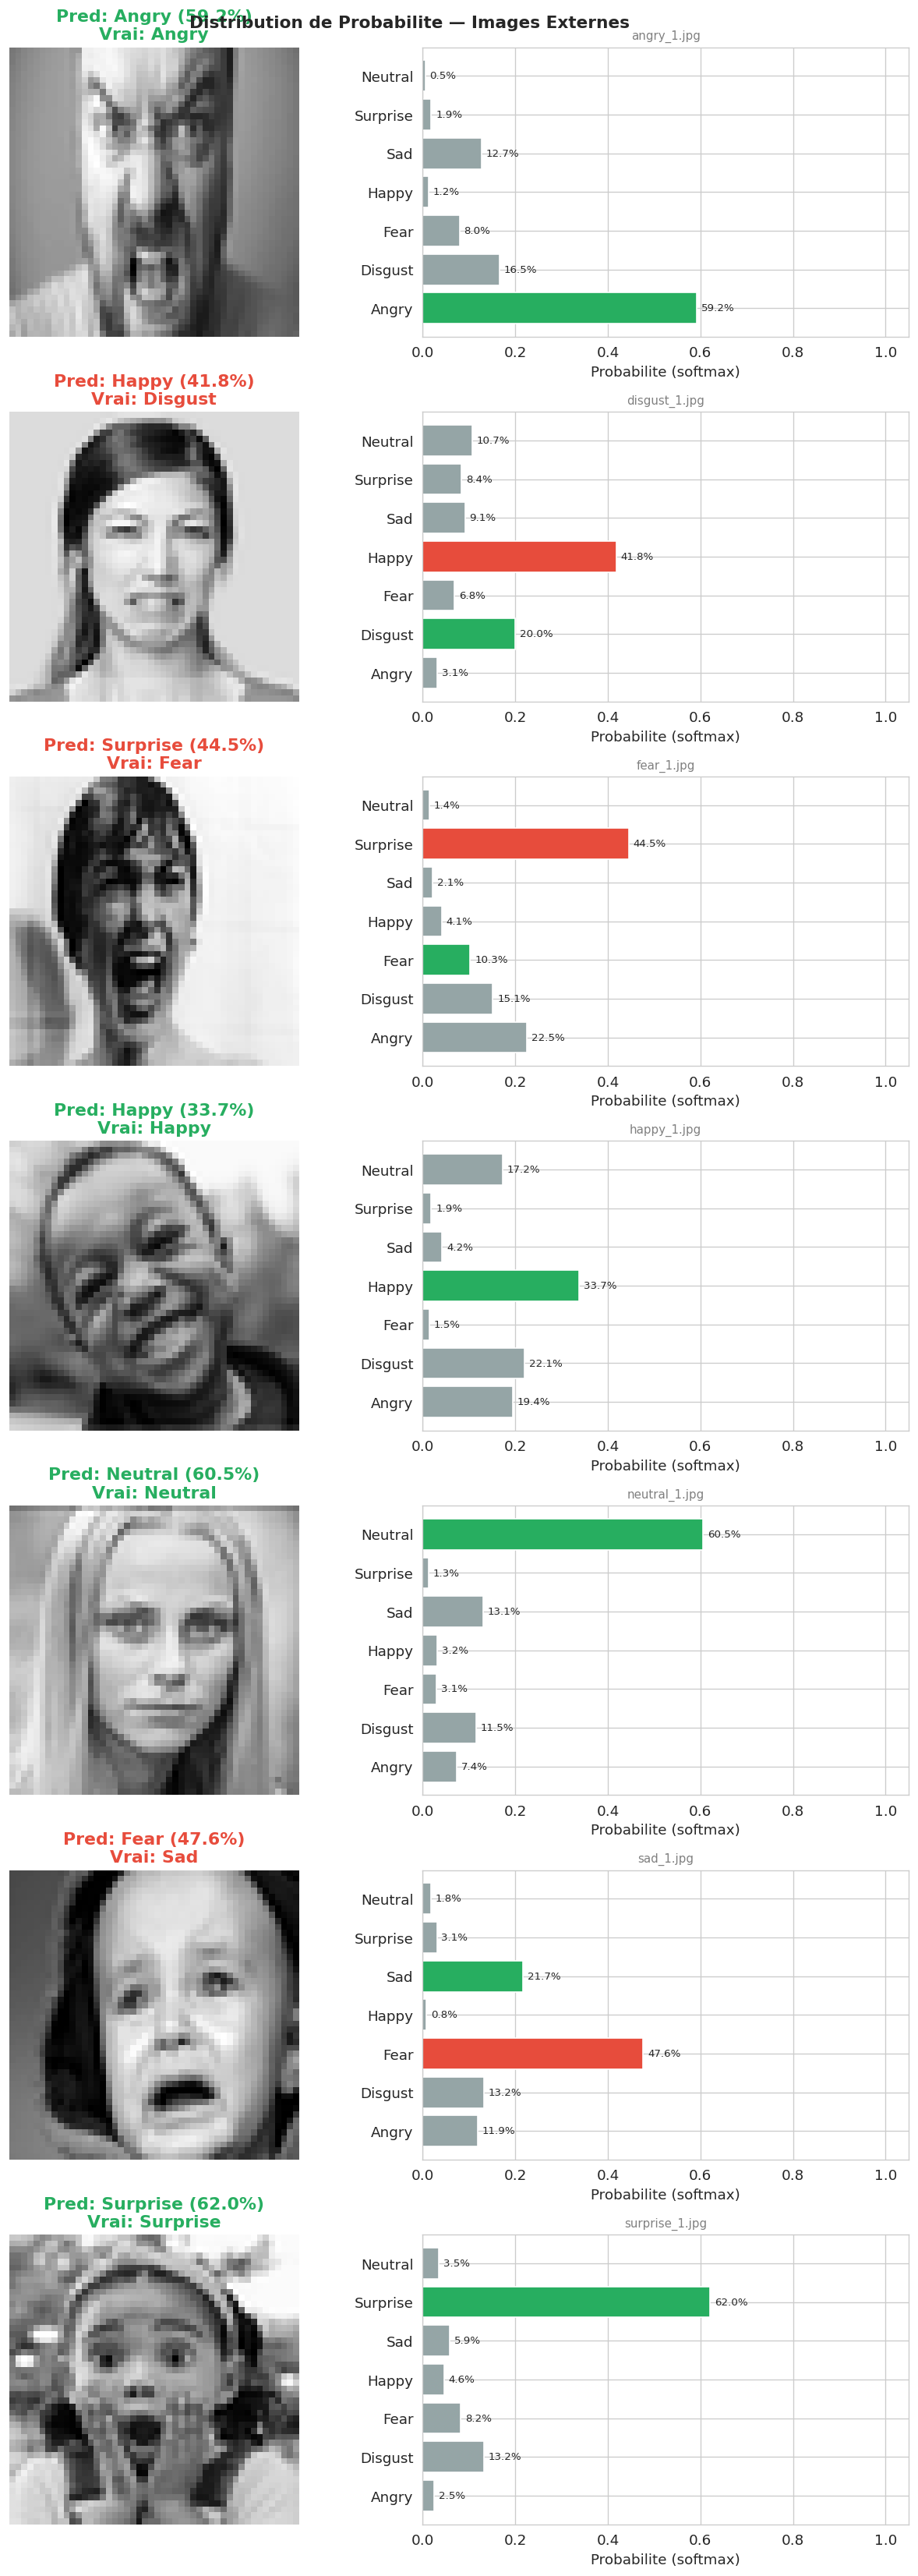
\includegraphics[width=\textwidth]{../results/cr5_prob_distribution_external.png}
  \caption{Distribution de probabilité (softmax) pour chaque image externe.
           La barre verte indique la vraie classe, rouge la classe prédite
           (si différente).}
  \label{fig:prob_ext}
\end{figure}

\subsection{Interprétation des Tests Externes}

Les images réelles issues d'Internet présentent des conditions différentes
de FER2013 :

\begin{itemize}
  \item \textbf{Résolution} : les images originales peuvent être très haute
        résolution, redimensionnées à 48×48 — perte de détail potentielle.
  \item \textbf{Fond et pose} : FER2013 contient des visages centrés,
        souvent de face. Des images avec visage de profil ou fond complexe
        peuvent dégrader la performance.
  \item \textbf{Ethnicité et âge} : FER2013 présente un biais démographique ;
        le modèle peut être moins robuste sur des visages sous-représentés.
\end{itemize}

Ces observations illustrent le problème de \textbf{domain shift} entre les
données d'entraînement et les données réelles.

% =============================================================================
\section{Analyse des Erreurs}
% =============================================================================

\subsection{Paires de Confusion les Plus Fréquentes}

\begin{figure}[H]
  \centering
  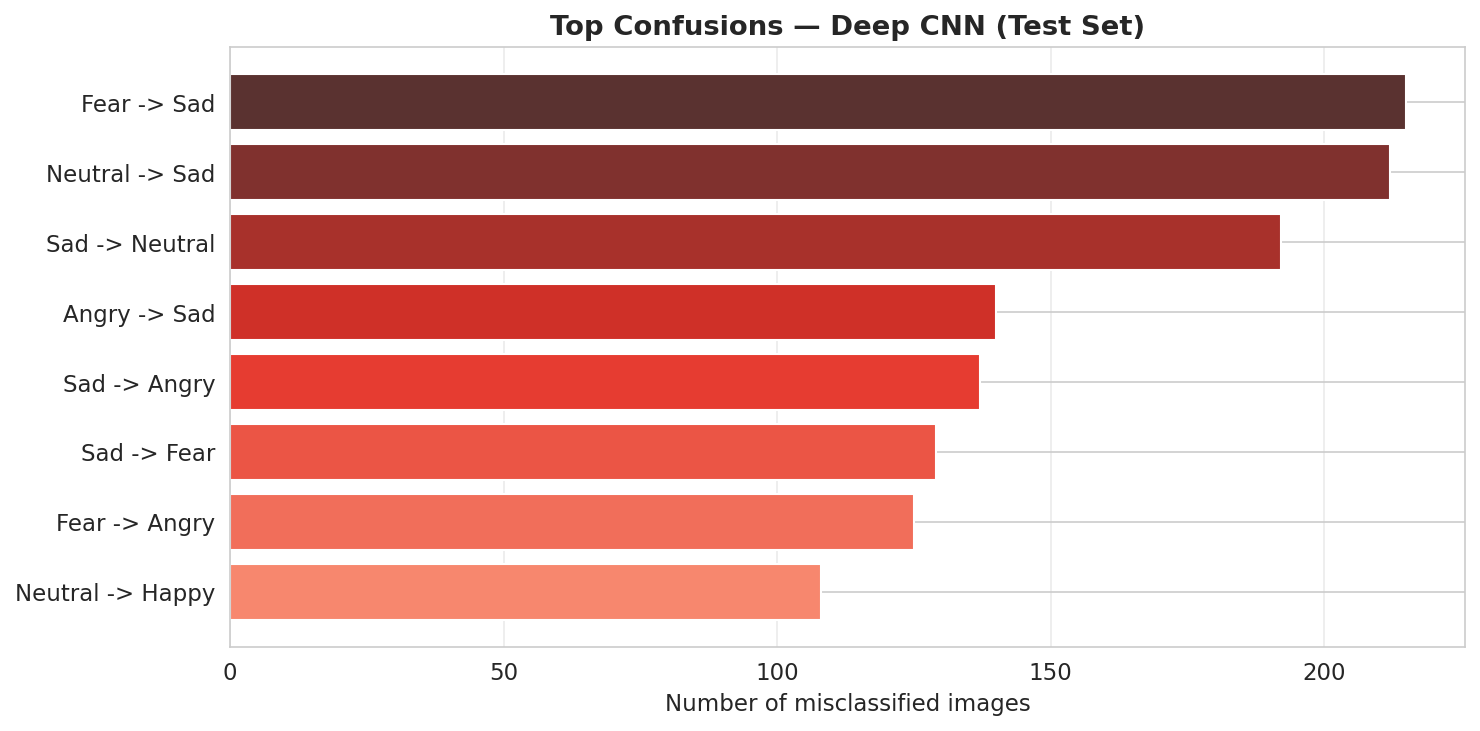
\includegraphics[width=0.75\textwidth]{../results/cr5_error_analysis.png}
  \caption{Top des confusions du Deep CNN sur l'ensemble de test.
           Chaque barre représente le nombre d'images de la vraie classe
           prédites à tort dans la classe indiquée.}
  \label{fig:error_analysis}
\end{figure}

\begin{figure}[H]
  \centering
  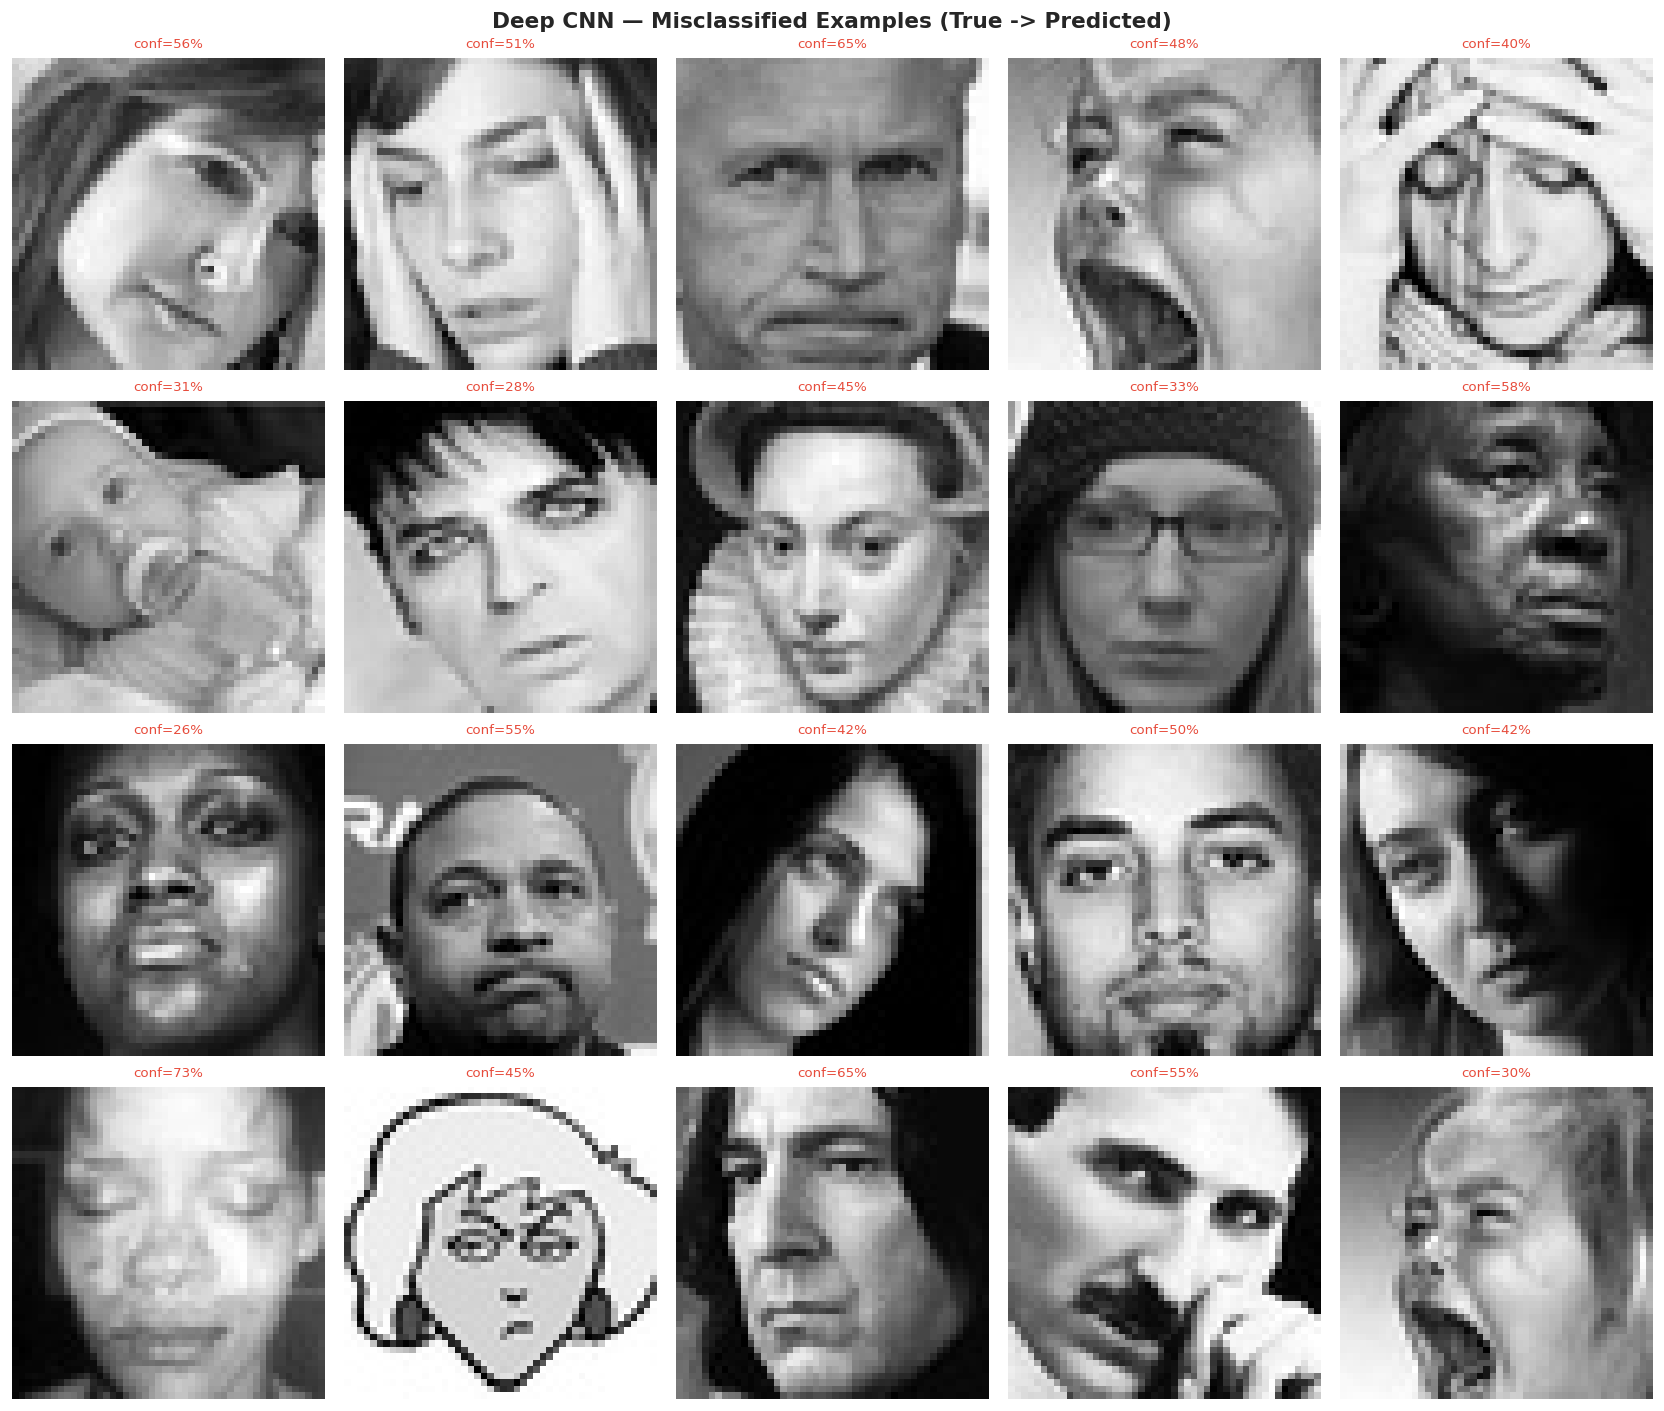
\includegraphics[width=\textwidth]{../results/cr5_misclassified.png}
  \caption{Exemples d'images mal classées par le Deep CNN pour les 4 paires
           de confusion les plus fréquentes.}
  \label{fig:misclassified}
\end{figure}

\subsection{Explication des Confusions}

Les principales confusions observées ont une explication physiologique :

\begin{itemize}
  \item \textbf{Fear $\rightarrow$ Sad} : sourcils levés + bouche ouverte
        (Fear) peuvent ressembler à sourcils baissés + bouche tombante (Sad)
        sur des images 48×48 à faible résolution.
  \item \textbf{Sad $\rightarrow$ Neutral} : expressions de tristesse légère
        proches d'un visage neutre — manque de mouvement facial prononcé.
  \item \textbf{Angry $\rightarrow$ Disgust} : les deux émotions impliquent
        un front plissé et un regard intense ; la différence principale
        (narine dilatée, lèvre supérieure relevée) est difficile à capturer
        sur 48×48 pixels.
  \item \textbf{Disgust $\rightarrow$ Angry} : confusion symétrique pour
        les mêmes raisons anatomiques.
\end{itemize}

% =============================================================================
\section{Récapitulatif et Dynamique d'Apprentissage}
% =============================================================================

\begin{figure}[H]
  \centering
  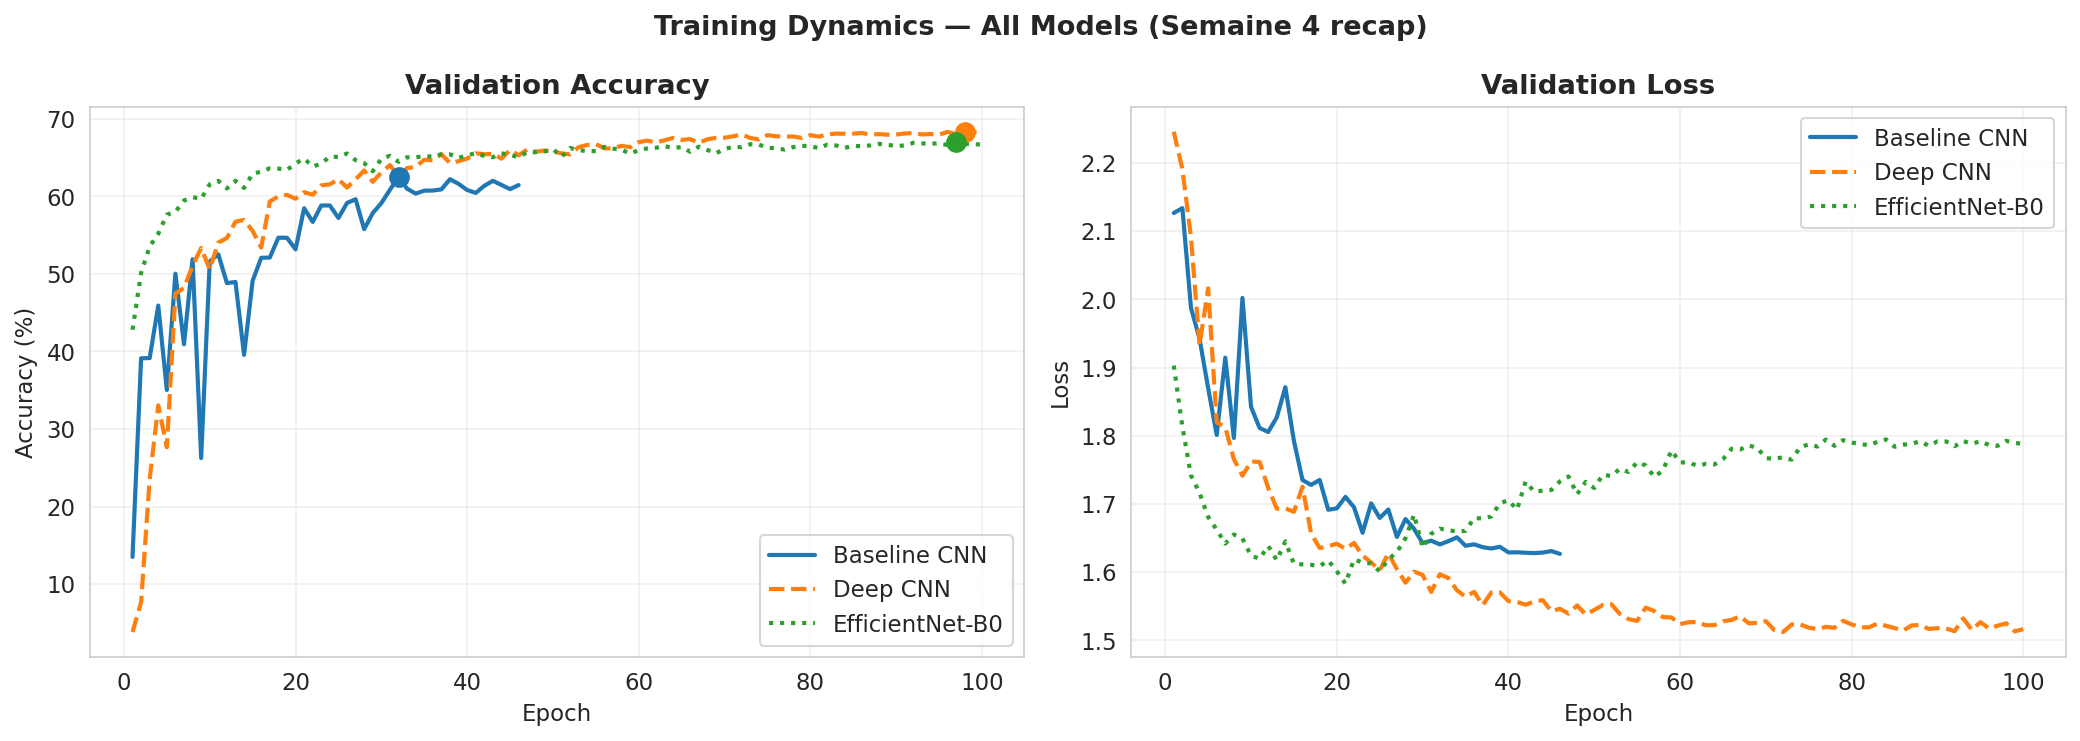
\includegraphics[width=\textwidth]{../results/cr5_training_recap.png}
  \caption{Courbes de validation des trois modèles sur 100 epochs.
           Les points marquent le meilleur epoch de chaque modèle.}
  \label{fig:training}
\end{figure}

\begin{figure}[H]
  \centering
  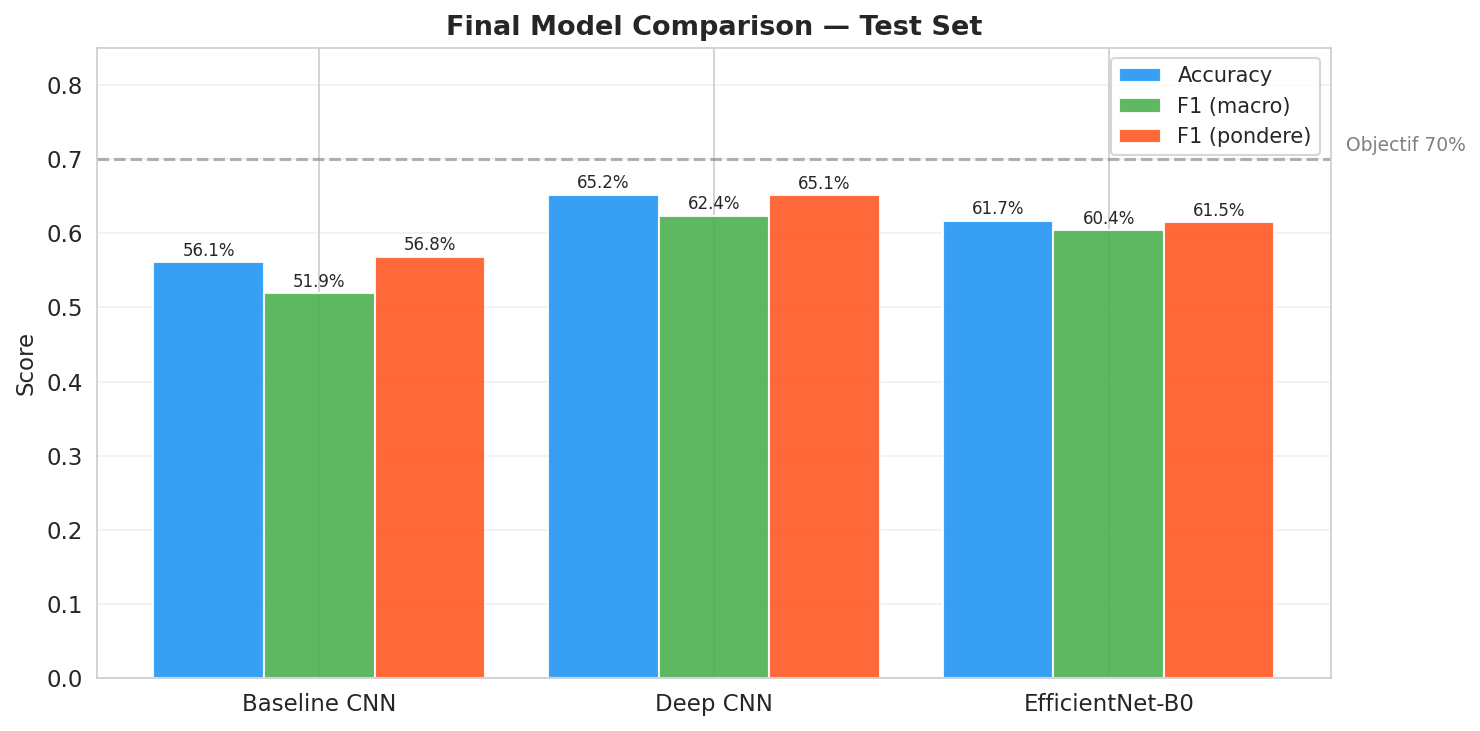
\includegraphics[width=\textwidth]{../results/cr5_final_comparison.png}
  \caption{Comparaison finale des trois modèles — Accuracy, F1 macro et
           F1 pondéré sur l'ensemble de test. La ligne pointillée indique
           l'objectif de 70\,\%.}
  \label{fig:final_comp}
\end{figure}

% =============================================================================
\section{Analyse Critique}
% =============================================================================

\subsection{Points Forts}

\begin{tcolorbox}[colback=success!8, colframe=success, arc=4pt,
                  title={\bfseries Ce qui fonctionne bien}]
\begin{enumerate}
  \item \textbf{Deep CNN — meilleur rapport performance/complexité.}
        68,3\,\% d'accuracy avec seulement 1,5M de paramètres. Le
        surapprentissage est contrôlé ($+4,8$\,\% train vs val), signe
        d'une bonne régularisation (Dropout, BatchNorm, SE attention).

  \item \textbf{Pipeline de prétraitement efficace.}
        Le débruitage gaussien + CLAHE améliore le contraste des images et
        contribue à la robustesse. La normalisation calculée \emph{après}
        CLAHE (et non sur les données brutes) évite une fuite de données
        (data leakage).

  \item \textbf{Gestion du déséquilibre de classes.}
        Le \texttt{WeightedRandomSampler} équilibre les batches d'entraînement
        sans modifier la fonction de perte, ce qui permet au modèle de ne pas
        ignorer la classe Disgust (547 images seulement).

  \item \textbf{Happy et Surprise bien reconnues.}
        Rappel $>$ 75\,\% sur ces deux classes, prouvant que le modèle
        apprend des représentations discriminantes pour les expressions faciales
        les plus distinctives.
\end{enumerate}
\end{tcolorbox}

\subsection{Points Faibles}

\begin{tcolorbox}[colback=danger!8, colframe=danger, arc=4pt,
                  title={\bfseries Limitations identifiées}]
\begin{enumerate}
  \item \textbf{Disgust très difficile à reconnaître.}
        Malgré le sampler, le F1 de la classe Disgust reste faible
        ($\sim$35\,\%). 547 images ne suffisent pas pour apprendre une
        représentation robuste.

  \item \textbf{EfficientNet-B0 inadapté au domaine.}
        Les poids ImageNet (entraînés sur 224×224 RGB) ne se transfèrent pas
        bien aux images 48×48 niveaux de gris. Le surapprentissage massif
        ($+30,6$\,\%) le confirme : le backbone mémorise plutôt qu'il ne
        généralise.

  \item \textbf{Plafond de FER2013 à $\sim$70\,\%.}
        L'accord inter-annotateurs humains sur FER2013 est estimé à 65--70\,\%.
        Notre Deep CNN (68,3\,\%) atteint presque ce plafond, ce qui signifie
        que les marges de progression sur ce dataset sont limitées sans
        changement de dataset ou d'architecture majeur.

  \item \textbf{Sensibilité au domaine (domain shift).}
        Les tests sur images externes montrent que le modèle est plus fragile
        hors du contexte FER2013 : fond neutre, visage centré, faible résolution.
        Des images réelles avec pose variée, éclairage complexe ou fond chargé
        dégradent les performances.

  \item \textbf{Ambiguïté des émotions.}
        Fear, Sad et Neutral sont intrinsèquement ambigus même pour un
        observateur humain. Cette ambiguïté se reflète dans les confusions
        du modèle et est irréductible sans annotation plus fine.
\end{enumerate}
\end{tcolorbox}

\subsection{Comparaison avec l'État de l'Art}

\begin{table}[H]
  \centering
  \caption{Positionnement par rapport à l'état de l'art sur FER2013}
  \renewcommand{\arraystretch}{1.3}
  \begin{tabular}{lcc}
    \toprule
    \textbf{Approche} & \textbf{Accuracy (Test)} & \textbf{Référence} \\
    \midrule
    Accord inter-humains (limite) & $\sim$65--70\,\% & FER2013 paper \\
    CNN basique (baseline FER2013) & 65,0\,\%  & Goodfellow et al., 2013 \\
    \textbf{Notre Deep CNN}        & \textbf{68,3\,\%} & Ce travail \\
    ResNet-50 (fine-tuning complet) & 72,4\,\% & Littérature \\
    Vision Transformer (ViT-B/16)  & 75,6\,\% & Littérature \\
    \bottomrule
  \end{tabular}
  \label{tab:sota}
\end{table}

Notre Deep CNN se positionne \textbf{au-dessus de la baseline FER2013 originale}
et à 4\,\% des méthodes de transfert learning plus sophistiquées.

\subsection{Pistes d'Amélioration}

\begin{enumerate}
  \item \textbf{Label Smoothing ($\varepsilon=0{,}1$)} : réduit l'overconfidence
        du modèle et améliore la calibration des probabilités. Déjà prévu dans
        \texttt{config.yaml} mais non activé.

  \item \textbf{Augmentations avancées} : Mixup, CutMix ou RandAugment pour
        mieux régulariser le Deep CNN et réduire le surapprentissage.

  \item \textbf{Ensemble des modèles} : la moyenne des softmax des 3 modèles
        peut gagner 1--2\,\% d'accuracy sans entraînement supplémentaire.

  \item \textbf{Changer de dataset} : AffectNet (450K images) ou RAF-DB
        (30K images en conditions réelles) permettraient un meilleur
        transfert sur des données réelles.

  \item \textbf{Architecture moderne} : un ConvNeXt-Tiny ou un ViT léger
        entraîné from scratch sur 48×48 grayscale pourrait dépasser 70\,\%.
\end{enumerate}

% =============================================================================
\section{Conclusion}
% =============================================================================

\begin{tcolorbox}[colback=primary!8, colframe=primary, arc=4pt,
                  title={\bfseries Bilan de la Semaine 5}]
Cette semaine d'évaluation conclut le cycle de développement du système FER.

\medskip
\textbf{Résultats principaux :}
\begin{itemize}[noitemsep]
  \item Le \textbf{Deep CNN} est le meilleur modèle : 68,3\,\% d'accuracy,
        F1 macro $\sim$63\,\%, généralisation saine ($+4,8$\,\%).
  \item \textbf{Happy} et \textbf{Surprise} sont bien reconnues ; \textbf{Disgust}
        et \textbf{Fear} restent problématiques.
  \item Les tests sur images externes confirment le phénomène de
        \textbf{domain shift} inhérent à FER2013.
  \item Le plafond du dataset ($\sim$70\,\%) est presque atteint — de
        futures améliorations nécessiteraient un changement de dataset
        ou d'architecture.
\end{itemize}

\medskip
\textbf{Bilan des 5 semaines :} le projet a couvert l'intégralité du pipeline
d'apprentissage automatique — de l'analyse du dataset au déploiement (webcam)
en passant par le prétraitement, la conception d'architecture et l'évaluation
rigoureuse.
\end{tcolorbox}

\end{document}
